\section{An identification-free pre-trade guard}\label{sec:guard}

\subsection{The quantity gate}
Observable dynamics are $z_{j+1}=Jz_j+Hv_j$ with loss output $l_t=Cz_t$, where $v_j$ is the executed quantity. Let $b_t=CJ^tz_0$ be the drift from past flow and $g_m=c^\top_{\rm price}J^mH$ the impulse coefficients. Which gain bounds the loss depends on the quantity contract. If quantities share a total budget over the window, $\sum_{j<t}|v_j|\le V$, the worst case of $|\sum_{m<t}g_mv_{t-1-m}|$ is $V\max_{m<t}|g_m|\equiv Vg^*_t$, attained by placing the whole budget at the lag of the peak, and execution costs at most $c_{\rm exec}V$. Under a reserve $L_{\rm other}$ the sharp allowance is then
\begin{equation}\label{eq:gate}
V^*=\min_{t:\,g^*_t+c_{\rm exec}>0}\frac{B-L_{\rm other}-|b_t|}{g^*_t+c_{\rm exec}},\qquad\bar R=V^*/\tau
\end{equation}
over a window of $\tau$ seconds. If instead each period's quantity is bounded, $|v_j|\le V$, the worst case is $V\sum_{m<t}|g_m|$ (attained by $v_{t-1-m}=V\,{\rm sign}(g_m)$) and execution costs at most $c_{\rm exec}Vt$, so the peak gain in \eqref{eq:gate} must be replaced by the summed gain $\sum_{m<t}|g_m|$ and $c_{\rm exec}$ by $c_{\rm exec}t$. Pairing a per-period bound with the peak gain understates the worst case, which is the failure Theorem~\ref{thm:guard} formalizes. Either gate needs only impulse coefficients and the current drift.

\subsection{Maximality}
A dealer with inventory $I$ chooses an admission level $\alpha\in[0,1]$ (the fraction of incoming algorithmic flow it accepts, or the depth it quotes). The closed-loop operator is $J(\alpha)=J_0+\alpha B_F$ with price impulse response $g_k(\alpha)$. Shocks satisfy $|u_t|\le\bar u$. Over horizon $H$ the price change is $\sum_{k<H}g_k(\alpha)u_{t-k}$, and the dealer has a loss budget $\mathcal B$. The contract is: inventory $I(\alpha)$ is held fixed over the horizon, each period's shock is bounded by $\bar u$, and loss is the mark-to-market loss at any date in the horizon; because the partial sums $\sum_{k<h}|g_k|$ increase in $h$, the worst date is the last. Margin, hedging and fills are added in Theorem~\ref{thm:forward}.

\begin{theorem}[Summed-gain guard is maximal]\label{thm:guard}
The worst-case loss over horizon $H$ is
\[
L_{\max}(\alpha)=|I(\alpha)|\,\bar u\sum_{k<H}|g_k(\alpha)|.
\]
Hence the guard ``admit $\alpha$ iff $L_{\max}(\alpha)\le\mathcal B$'' is necessary and sufficient for bounded-shock solvency: it admits every safe $\alpha$ and no unsafe one. Replacing $\sum_k|g_k|$ by $\max_k|g_k|$ can admit unsafe levels; replacing it by $H\max_k|g_k|$ is safe but conservative.
\end{theorem}

\begin{proof}
By H\"older's inequality $|\sum_kg_ku_{t-k}|\le\bar u\sum_k|g_k|$, with equality for $u_{t-k}=\bar u\,{\rm sign}(g_k)$, which is admissible. Multiplying by $|I(\alpha)|$ gives $L_{\max}$, so the admission set equals the safe set. Since $\max_k|g_k|\le\sum_k|g_k|\le H\max_k|g_k|$, the peak guard under-states loss and the $H$-scaled guard over-states it.
\end{proof}

The worst-case identity in Theorem~\ref{thm:guard} is not new as mathematics: the induced $\ell_\infty$ gain of a linear convolution operator is the $\ell_1$ norm of its kernel, the fact on which $\ell_1$-optimal control of persistent bounded disturbances is built \citep{vidyasagar1986,dahleh1987,dahleh1995}. We use it rather than claim it. The finance content lies elsewhere: the dealer's admission level changes the operator itself, so the guard is a rule over an action set rather than a controller design; the bound is carried through margin, hedging and fill accounting (Theorem~\ref{thm:forward}); its single input is invariant to how the unobserved traders are split into cohorts and is identified from prices (Propositions~\ref{prop:invariance} and~\ref{prop:bridge}); the peak-response and eigenvalue rules it is compared with are the ones closest to current supervisory practice; and the same statistic prices the corrective rebate in equilibrium (Proposition~\ref{prop:equil}).

Numerically, the guard coincides with a brute-force adversary's maximal safe $\alpha$ in 200 of 200 random states. The peak-gain guard admitted an unsafe level in 2,000 of 2,000 states, the $H$-scaled guard was conservative in all 2,000, and $L_{\max}$ was non-decreasing in $\alpha$ in all 2,000, so the admission set was an interval in these examples.

\subsection{Computability: a finite-horizon certificate}

\begin{lemma}[Contraction-block tail bound]\label{lem:tail}
Let $\rho(J(\alpha))<1$. Suppose that at horizon $H$ there is a block length $H_0\le H$ with $q(\alpha)\equiv\|J(\alpha)^{H_0}\|_2<1$, and let $\bar M_{H_0}(\alpha)=\max_{0\le r<H_0}\|c^\top_{\rm price}J(\alpha)^r\|_2$ and $M_{C,H}(\alpha)=\max_{k\le H}\|c^\top_{\rm price}J(\alpha)^k\|_2$. Then
\begin{align}
\sup_{k\ge0}\|c^\top_{\rm price}J(\alpha)^k\|_2&\le\max\Bigl(M_{C,H}(\alpha),\ \bar M_{H_0}(\alpha)q(\alpha)^{\lfloor(H+1)/H_0\rfloor}\Bigr),\label{eq:tail}\\
G_{{\rm cum},\infty}(\alpha)&\le G_{{\rm cum},H}(\alpha)+\frac{\bar M_{H_0}(\alpha)H_0\,q(\alpha)^{\lfloor(H+1)/H_0\rfloor}}{1-q(\alpha)}.\notag
\end{align}
\end{lemma}

\begin{proof}
Write any $k>H$ as $k=mH_0+r$ with $m\ge\lfloor(H+1)/H_0\rfloor$ and $0\le r<H_0$. Submultiplicativity gives $\|c^\top J^k\|\le\|c^\top J^r\|\,\|J^{H_0}\|^m\le\bar M_{H_0}q^m$. Taking the supremum and summing the geometric tail gives \eqref{eq:tail}.
\end{proof}

The certificate turns an infinite-horizon supremum into a finite computation with a verified remainder. If the second term in the maximum is below $M_{C,H}$, truncation at $H$ is exact.

Example~\ref{ex:witness} shows why the certificate is needed: two economies can agree exactly on the first coefficients and still differ threefold in their summed response.

\subsection{Robustness to estimation error}

\begin{theorem}[Robust gain]\label{thm:robust}
Let $M=\sup_k\|J^k\|$ and $S=\sum_k\|J^k\|$. If $\|E\|\le\epsilon$ and $\epsilon S<1$, then $\sup_k\|(J+E)^k\|\le M/(1-\epsilon S)$.
\end{theorem}

\begin{proof}
Let $P_k=(J+E)^k$. Expanding, $P_k=J^k+\sum_{j<k}J^{k-1-j}EP_j$. With $m_k=\|P_k\|$, $m_k\le M+\epsilon\sum_{j<k}\|J^{k-1-j}\|m_j\le M+\epsilon S\max_{j<k}m_j$. Since $m_0=1\le M$, induction gives $m_k\le M/(1-\epsilon S)$ for all $k$.
\end{proof}

Theorem~\ref{thm:robust} is deterministic: it holds whenever $\|E\|\le\epsilon$. A statistical guarantee follows only through a confidence set for the operator, and then holds with that set's coverage probability, not with certainty. The bound held in all 30,000 random perturbations of 100 non-normal operators, with median tightness $0.50$ (realized gain over bound; maximum $0.57$). In a simulated window estimator of the kind used in Section~\ref{sec:spot} (600 transitions), a residual-bootstrap 95\% ball for the operator covered the true $J$ in $94.7\%$ of 300 replications, with median radius $0.086$; but $\epsilon S<1$ held in only $8\%$ of windows. The certificate is valid but often unavailable at realistic sample sizes; longer windows or pooled estimates are needed to use it in practice.

\begin{proposition}[No identification needed; numerical]\label{prop:bridge}
In a two-cohort economy with rates $0.7\pm\Delta$, the relative error of the estimated summed gain is flat in $\Delta$ (log--log slope $-0.15$), while the error of the cohort weights grows as $\Delta^{-3.07}$.
\end{proposition}

The guard needs the summed gain, which is cheap to estimate and invariant to cohort splitting (Proposition~\ref{prop:invariance}); it does not need the algorithms' identities, which are expensive \citep{niroula2026}.


\subsection{An uncertainty-aware guard}\label{sec:robustguard}
The guard of Theorem~\ref{thm:guard} assumes the operator is known. With data, the relevant question is which admission levels are safe for every economy the data allow. We answer it for a venue gate (Mode B below) in the positive cohort economy, where admitting a fraction $\alpha$ of the algorithmic flow scales every cohort's weight, $M\mapsto\alpha M$, so that $S(\alpha)=\kappa/(1-a-\kappa\alpha\Phi)$.

\begin{lemma}[Soundness of compatible-set guards]\label{lem:sound}
If a data-dependent set $\mathcal C(D)$ contains the true economy with probability at least $1-\gamma$, then every action whose worst-case loss is within budget for all economies in $\mathcal C(D)$ is within budget for the true economy with probability at least $1-\gamma$, including an action selected from the data. If no action qualifies, the guard certifies nothing: it halts new admission and flags the state, because existing inventory can be unsafe even with no new trading.
\end{lemma}

\begin{theorem}[Optimal uncertainty-aware admission]\label{thm:robustguard}
Let position $I$, shock bound $\bar u$ and budget $\mathcal B$ be given, and let $\Phi^+$ be an upper bound on $\Phi$ valid with probability at least $1-\gamma$ (for example $\Phi^+=(1-a-\kappa/\hat S^+)/\kappa$ from Theorem~\ref{thm:certcost}, or $\Phi_+$ from Theorem~\ref{thm:window}). Put $c_I=1-a-\kappa|I|\bar u/\mathcal B$.
\begin{enumerate}[label=(\roman*)]
\item \emph{Closed form and interval.} If $c_I\ge0$, the levels that are safe for every $\Phi\le\Phi^+$ form the interval $[0,\alpha^*]$ with $\alpha^*=\min\{1,\ c_I/(\kappa\Phi^+)\}$.
\item \emph{Safety.} With probability at least $1-\gamma$, every admitted level is safe for the true economy.
\item \emph{Maximality.} Every level above $\alpha^*$ is unsafe for an economy with $\Phi=\Phi^+$; when $\Phi^+$ is attained by a compatible economy (as for $\Phi_+$ in Theorem~\ref{thm:window}), no rule using the same information can admit more without admitting an unsafe level.
\item \emph{Infeasibility.} If $c_I<0$, no level is safe, including $\alpha=0$: the guard halts admission and the position must fall to $|I|\le\mathcal B(1-a)/(\kappa\bar u)$.
\item \emph{Minimax capacity loss.} On the class of Theorem~\ref{thm:certcost} with $\Phi$ bounded away from zero, the certificate-based guard gives up $\alpha^\circ-\alpha^*=O\bigl(\sigma\sqrt{\log N/N}\bigr)$ of the oracle capacity $\alpha^\circ=\min\{1,c_I/(\kappa\Phi)\}$ with probability at least $1-2\gamma$, and every rule that admits an unsafe level with probability at most $\beta<1$ gives up at least $c\,\sigma/\sqrt N$ in expectation at some economy of the class. The guard is minimax-optimal in lost capacity up to a logarithmic factor.
\end{enumerate}
\end{theorem}

Monotonicity of $S(\alpha)$ in $\alpha$ and $\Phi$ gives (i)--(iv); (v) combines the certificate's excess with Proposition~\ref{prop:twoworld} applied to two economies whose capacities differ by order $\sigma/\sqrt N$ (Appendix~\ref{app:proofs}). In 500 random economies the closed form matched a brute-force search over 1{,}001 admission levels, computed from the state matrices rather than from \eqref{eq:SPhi}, in every case; every safe set was an interval; and the 28 infeasible states were flagged (test T06). Across 18 designs the certificate covered the true summed response at least at its nominal level (minimum 93.6\% at nominal 90\%), with a median excess of 3--15\% when the memory bound is $0.6$ or $0.9$ and about 230\% when it is $0.97$, where the tail term dominates (test T04).

\subsection{A calibrated illustration}\label{sec:calib}

How much does the choice between peak and summed guards matter in a real book? We compute the three-state impulse response at the median estimates of Section~\ref{sec:depth} (all training days and high-volatility days) and at a hypothetical book in which flow depletes the side it hits ($\varepsilon=+0.02$, other parameters at their high-volatility medians), Figure~\ref{fig:calib} and Table~\ref{tab:calib}.

\begin{figure}[t]\centering
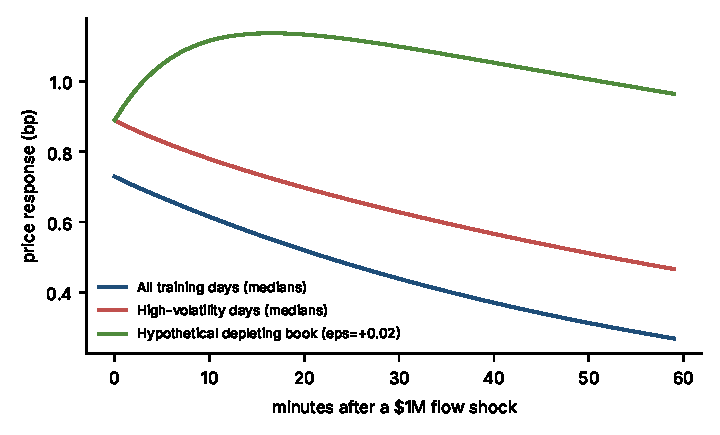
\includegraphics[width=0.62\textwidth]{figs/fig_calib.pdf}
\caption{Price response to a \$1M flow shock at the median depth estimates and in a hypothetical depleting book. Computed from the estimates of Table~\ref{tab:d3}.}\label{fig:calib}
\end{figure}

\begin{table}[t]\centering\small
\begin{threeparttable}
\caption{Peak versus summed gain at calibrated parameters}\label{tab:calib}
\setlength{\tabcolsep}{4pt}
\begin{tabular}{p{0.2\textwidth}ccccccc}
\toprule
Book & $C_3$ & Peak (min) & $\sum_{k<15}|g_k|$ & $\sum_{k<60}|g_k|$ & Sum/peak & Cap, peak & Cap, sum\\
\midrule
All days (medians) & $-0.013$ & 0.73 (0) & 9.73 & 27.67 & 13.3 & \$274M & \$21M\\
High-vol.\ days (medians) & $-0.014$ & 0.89 (0) & 12.17 & 38.71 & 13.7 & \$225M & \$16M\\
Depleting book ($\varepsilon=0.02$) & $+0.042$ & 1.14 (17) & 15.85 & 63.69 & 14.0 & \$176M & \$13M\\
\bottomrule
\end{tabular}
\begin{tablenotes}\footnotesize\item Gains in bp per \$1M of flow; sum/peak at 15 minutes. Inventory cap under a peak guard and under the summed guard, for a loss budget of \$100,000, an illustrative shock bound of \$5M of flow per minute and a 15-minute horizon. From \texttt{calib\_guard.py}, using the medians of Table~\ref{tab:d3}.\end{tablenotes}
\end{threeparttable}
\end{table}

The result is striking even though BTCUSDT does not amplify. Because price impact is persistent ($\hat a\approx0.97$ per minute), the summed gain over 15 minutes is about 13 times the peak. A guard calibrated to the peak would admit inventory about 13 times larger than is safe against a sustained adversarial flow of the declared size. Amplification makes this worse (the depleting book peaks 17 minutes after the shock), but persistence alone already makes peak-based limits unsafe. This is the practical content of Theorem~\ref{thm:guard} for this market.

\subsection{Two deployment modes}

\begin{enumerate}[label=\textbf{Mode \Alph*.},leftmargin=*]
\item \emph{An individual dealer.} A price-taking market maker with a small share of aggregate depth scales its own quote size by $\alpha$. This scales its passive fill intake but leaves aggregate depth, impact and the market operator unchanged.
\item \emph{A venue or sponsoring broker.} A gate at a matching engine or a market-access gateway (the setting of Rule 15c3-5) admits a fraction $\alpha$ of incoming aggressive algorithmic flow while resting depth stays posted. The operator becomes $J(\alpha)=A_0+\alpha B_F$.
\end{enumerate}

\paragraph{Algorithm (pre-trade guard).} At each step, using only pre-shock information:
\begin{enumerate}[itemsep=1pt]
\item For each $\alpha$ on a grid $\mathcal A=\{0,0.025,\ldots,1\}$, compute $\rho(J(\alpha))$, the peak and summed gains $M_{C,H}(\alpha)$ and $G_{{\rm cum},H}(\alpha)$, and the tail certificate of Lemma~\ref{lem:tail}; if an operator confidence radius $\epsilon$ is available, inflate by Theorem~\ref{thm:robust}.
\item Compute post-hedge and worst-case post-fill inventory, hedging cost and the post-fill margin increment.
\item Admit the largest $\alpha\in\mathcal A$ that satisfies the solvency inequalities of Theorem~\ref{thm:forward}; if none does, set $\alpha=0$, flag that no safe action exists, and trigger inventory reduction.
\end{enumerate}
The guard checks every grid point, so it does not rely on the safe set being an interval; levels between grid points are never admitted. For low-dimensional $J$ the grid evaluation is a sequence of matrix--vector products; execution takes well under one millisecond in compiled code, which we regard as an engineering detail rather than a result.

\subsection{Balance-sheet solvency}

\begin{theorem}[Conditional bounded-shock forward solvency]\label{thm:forward}
Consider a dealer with cash $K_t$, inventory $I_t$, mark $p_t$, equity $E_t=K_t+I_tp_t$, maintenance margin $MM_t=\max(0,\mu|I_t|p_t-c_0)$ and remaining buffer $B_{{\rm rem},t}=E_t-MM_t$, a safety reserve $R_{\rm safe}$, a hedge $\Delta I^{\rm hedge}_t(\alpha)$ with cost $C_{{\rm hedge},t}(\alpha)$, worst-case passive fills $\Delta I^{\rm fill}_{\max,t}(\alpha)$ with margin increment $C_{{\rm fill},t}(\alpha)$, and declared one-step and cumulative shock envelopes $\bar u_{{\rm step},t}\le\bar u_{{\rm cum},t}$. Let $|I^{\rm post}_{t+1}(\alpha)|=|I_t+\Delta I^{\rm hedge}_t(\alpha)|+\Delta I^{\rm fill}_{\max,t}(\alpha)$. Suppose the guard admits $\alpha_t$ only if
\begin{equation}\label{eq:guardineq}
|I^{\rm post}_{t+1}(\alpha_t)|(1+\mu)\Bigl(M_{C}(\alpha_t)\|z_t\|_2+s(\alpha_t)G_{\rm cum}(\alpha_t)\bar u_{{\rm cum},t}\Bigr)+C_{{\rm hedge},t}(\alpha_t)+C_{{\rm fill},t}(\alpha_t)+R_{\rm safe}\le B_{{\rm rem},t},
\end{equation}
where $s(\alpha)$ scales admitted shocks. Then for every disturbance path within the declared envelopes, the buffer after the step is at least $R_{\rm safe}$; by induction, solvency holds at every step at which an admissible $\alpha$ exists. At $\alpha=0$ the one-step admissible shock is
\[
\bar u_{{\rm adm},t}=\frac{B_{{\rm rem},t}-R_{\rm safe}-|I_t|(1+\mu)\|z_t\|_2}{|I_t|(1+\mu)} .
\]
The condition is sufficient over the whole disturbance ball. It is also necessary when the current state contributes no drift ($z_t=0$), because the shock term is then attained by adversarially signed disturbances; with $z_t\neq0$ the drift term $M_C\|z_t\|_2$ is an upper bound and the condition may be conservative. The admissible shock at $\alpha=0$ assumes, as in the cohort economy (Lemma~\ref{lem:cm}), that the price-row gain without admitted flow is $M_C(0)=1$.
\end{theorem}

Two features matter. The guard accounts for the inventory the dealer will hold after hedging and after worst-case fills, not only current inventory, and it never claims safety on an infeasible state: if no $\alpha$ satisfies \eqref{eq:guardineq}, it halts new fills and flags the state, because pre-existing inventory can still breach margin on a large adverse jump. In a constructed scenario ($E_0=10{,}000$, $I_0=-2{,}000$ at $P^*=100$, Tier-2 margin with $\mu=0.005$, buffer $9{,}050$ and reserve $950$), the admissible shock at $z_0=0$ is $8{,}100/2{,}010=4.03$ per unit, and an adversarial move of $4.05$ violates the reserve.

\begin{proposition}[When an eigenvalue rule admits an uncertified level]\label{prop:dominance}
Let an eigenvalue guard admit $\alpha_\rho=\max\{\alpha:\rho(J(\alpha))\le\bar\rho\}$, and suppose the state is feasible for the summed-gain guard, which then admits at least $\alpha=0$. Bounding the one-step price move by $M_C(\alpha)(\|z_t\|_2+s(\alpha)\bar u_{{\rm step},t})$, the level admitted by the eigenvalue guard fails this one-step solvency certificate, and so is one the summed-gain guard would not certify, if and only if
\[
M_C(\alpha_\rho)\;>\;\frac{B_{{\rm rem},t}-R_{\rm safe}-C_{{\rm hedge},t}(\alpha_\rho)-C_{{\rm fill},t}(\alpha_\rho)}{|I^{\rm post}_{t+1}(\alpha_\rho)|(1+\mu)(\|z_t\|_2+s(\alpha_\rho)\bar u_{{\rm step},t})} .
\]
\end{proposition}

The certificate is a bound, so failing it means that solvency cannot be guaranteed, not that a breach must occur. The eigenvalue rule fails it exactly when the transient gain at its admitted level exceeds the loss the balance sheet can absorb, which Proposition~\ref{prop:blind} shows can happen at any spectral threshold.

\begin{proposition}[Strategic re-optimization reinforces the guard]\label{prop:lucas}
Suppose cohorts re-optimize their steady-state Kalman gains when the venue throttles admission, and throttling scales the variance of execution-driven innovations as $\sigma_\zeta^2(\alpha)=\alpha^2\sigma_{\zeta,0}^2$ while measurement noise $\sigma_\nu^2>0$ is unchanged. Then the optimal gain $\eta^*(\alpha)$ is strictly increasing in $\alpha$, so throttling lowers every cohort's adaptation rate. If the transient gain is non-decreasing in the adaptation rates, then $M_C(J(\alpha,\eta^*(\alpha)))\le M_C(J(\alpha,\eta^*(1)))$: re-optimization does not undo the guard.
\end{proposition}

The first statement is a property of the Riccati root; the second is conditional on monotonicity of the gain in $\eta$, which we check numerically. Across 3{,}000 stable draws of the three-state book with momentum (adaptation rates on a grid from 0.05 to 0.95), the peak response is non-decreasing in $\eta$ in 98.8\% of draws and in 99.9\% of those with trend-following cohorts ($q>0$); the summed absolute response is non-decreasing in 93\% of draws with $q>0$ but decreasing when cohorts are contrarian ($q<0$). For trend-following cohorts, the case the filtering microfoundation produces, re-optimization therefore reinforces the guard in almost every case we drew; the signed sum $S$ of Proposition~\ref{prop:sum} does not depend on $\eta$ at all (\texttt{recompute\_oct20.py}). A manipulator who instead increases order size to offset throttling enlarges the shock envelope and drives $\alpha$ toward zero.
